% Presentation 3 (June 26): Progress / Results. 
% Focus on things done and Sensitivity Analysis

% \begin{frame}
%     \frametitle{ }
%     \begin{quote}
%         \centerline{In 30 minutes\ldots}
%         \vskip 16pt
%         \centerline{you'll know how to be financially sophisticated}
%         \centerline{and profit from the financially na\"{i}ve!}
%     \end{quote}
% \end{frame}


\begin{frame}{Outline}
    \tableofcontents
\end{frame}

\section{Introduction}

\begin{frame}{Recap}
    % Reminder of what I was planning to do 
        \begin{itemize}
            \item {\bf Goal}: Recommend an optimized credit card portfolio, based on user income/spend and preferences, and study its properties
            \bigskip
            \item {\bf Last Week}: Credit Card and Budget Data
            \bigskip
            \item {\bf This Week}: Results 1/2
            \begin{itemize}
                \item Algorithm
                \item Sensitivity Analysis
            \end{itemize}
            \bigskip
            \item In {\bf Two Weeks}: Results 2/2
            \begin{itemize}
                \item Monte Carlo Simulations
                \item Shiny App
            \end{itemize}
        \end{itemize}
    \end{frame} 
    

\section{Algorithm}

\begin{frame}{Two \sR\ Functions}
    \begin{enumerate}
        \item \texttt{get\_budget}: returns a budget based on income 
        \item \texttt{get\_portfolio}: returns a portfolio (card names, net benefit, marginal benefit, return-on-spend, total spend, and which card to use for which category) 
        \begin{itemize}
        \item 0. Calculate ``spend matrix'': $y_{kc} = x_{kc}\/m_{kc}( \eta\/ v_{t,k} + 
            (1 - \eta)\/ v_{b,k})$ 
        \item 1. Calculate row sums:
        \[
            \sum_{c=1}^{18} y_{kc} + \theta\/ b_{k} - f_{k}
        \]
        \item 2. Select highest value card, store its name, net benefit, marginal benefit, and spend categories
        \item 3. Subtract its values from all cards in the matrix (set negative values to 0)
        \item 4. Set the benefits of the selected card to 0! (avoids reselection)
        \item Go to step 1 ($K$ times for $K$ cards)
        \end{itemize}
    \end{enumerate}
\end{frame} 



\begin{frame}{Tweaked Credit Card Dataset}
    % Addressed duplicate cards and how to remove cards after first selection
    \begin{itemize}
        \item Find duplicates of selected card by ID number
    \end{itemize}
    \begin{center}
        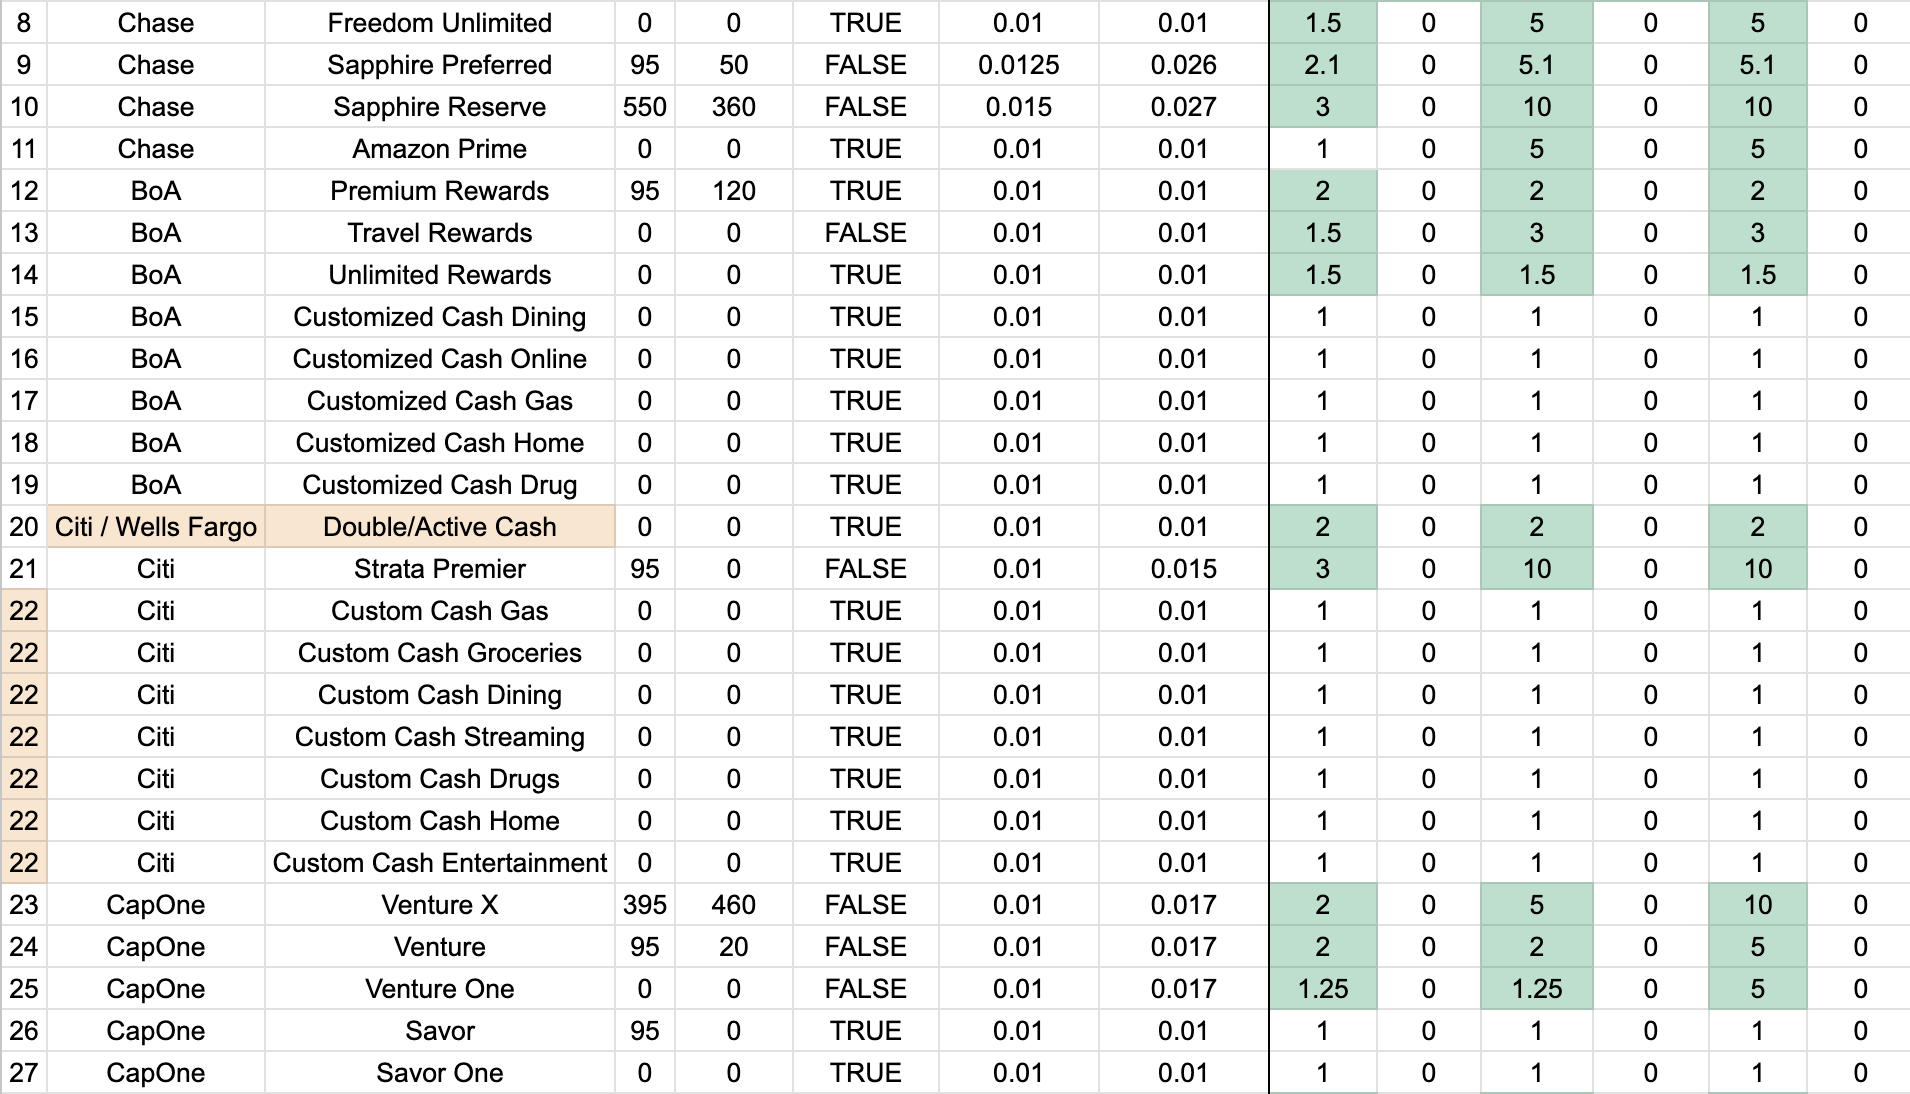
\includegraphics[width=1\textwidth]{../Misc/CreditCardsUpdate.png}
    \end{center}
\end{frame} 


\begin{frame}{\sR\ Code for \texttt{get\_budget}}
        \begin{columns}[c]
            \begin{column}{0.65\textwidth}
                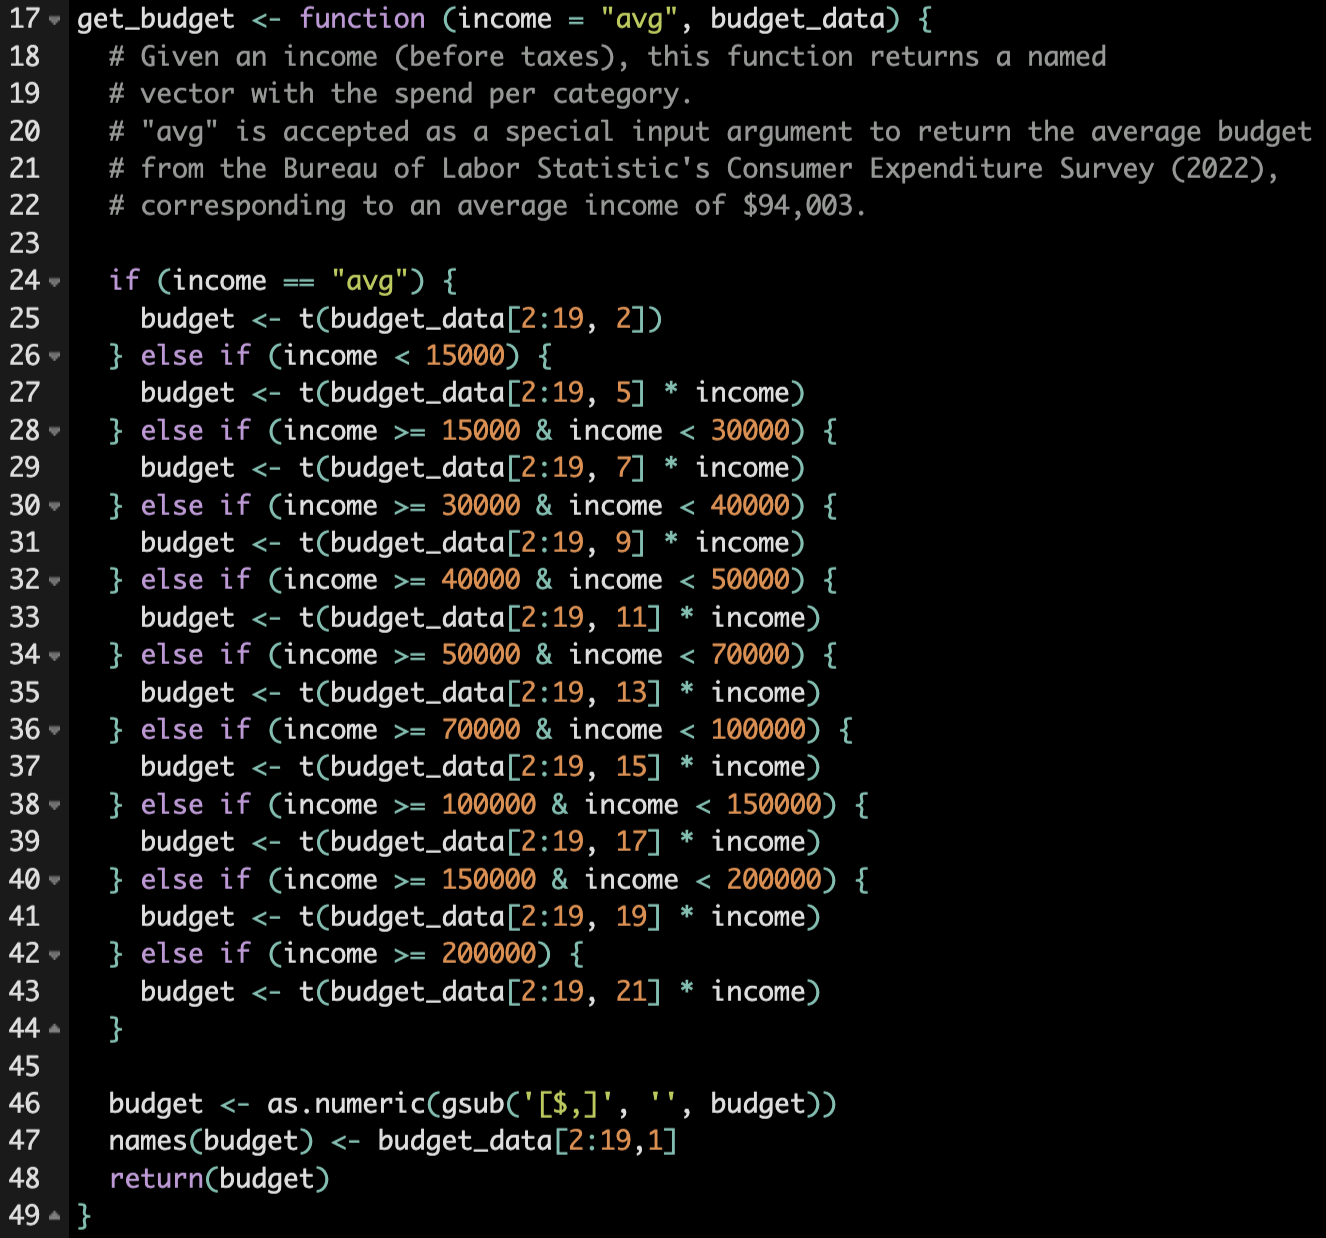
\includegraphics[height=0.8\textheight]{../Misc/RCode_budget1.png}
            \end{column}
            \begin{column}{0.3\textwidth}
                    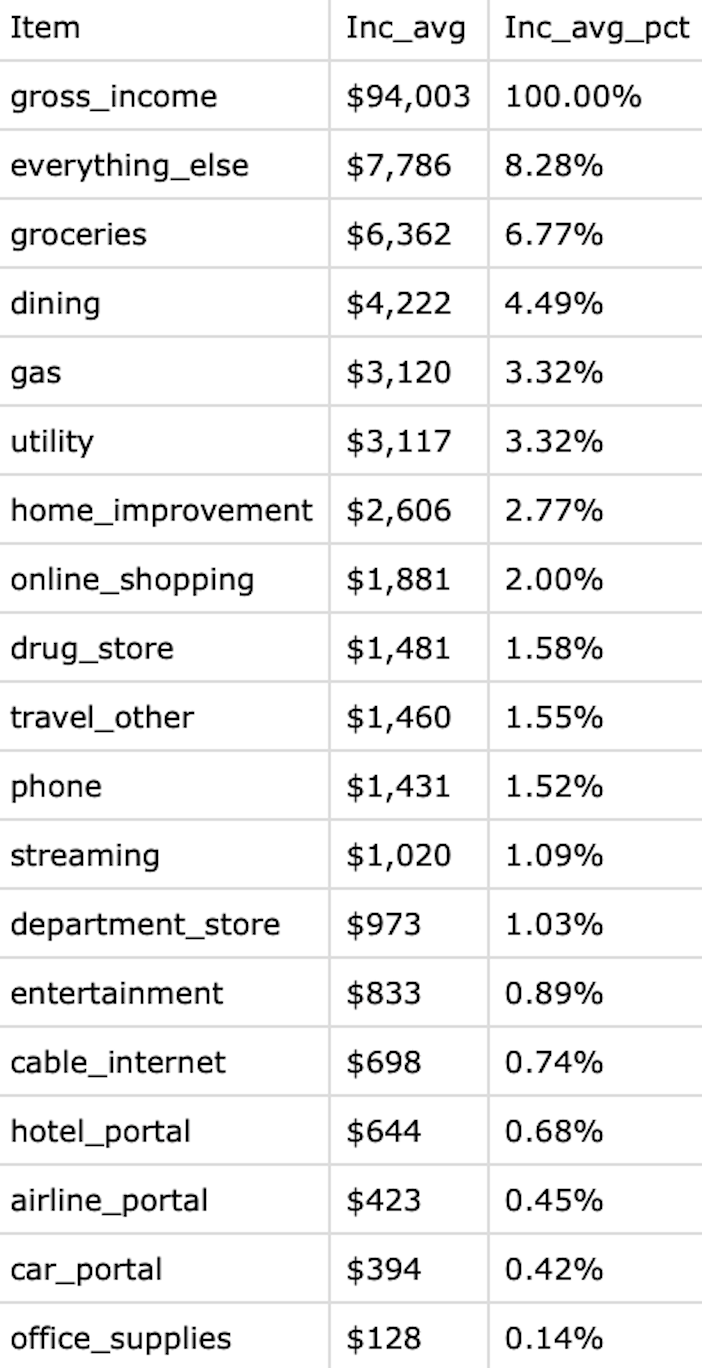
\includegraphics[height=0.8\textheight]{../Misc/RCode_budget2.png}
            \end{column}
        \end{columns}
\end{frame} 

\begin{frame}{\sR\ Code output for \texttt{get\_portfolio}}
    \begin{itemize}
        \item Conservative user input
    \end{itemize}
    \begin{center}
        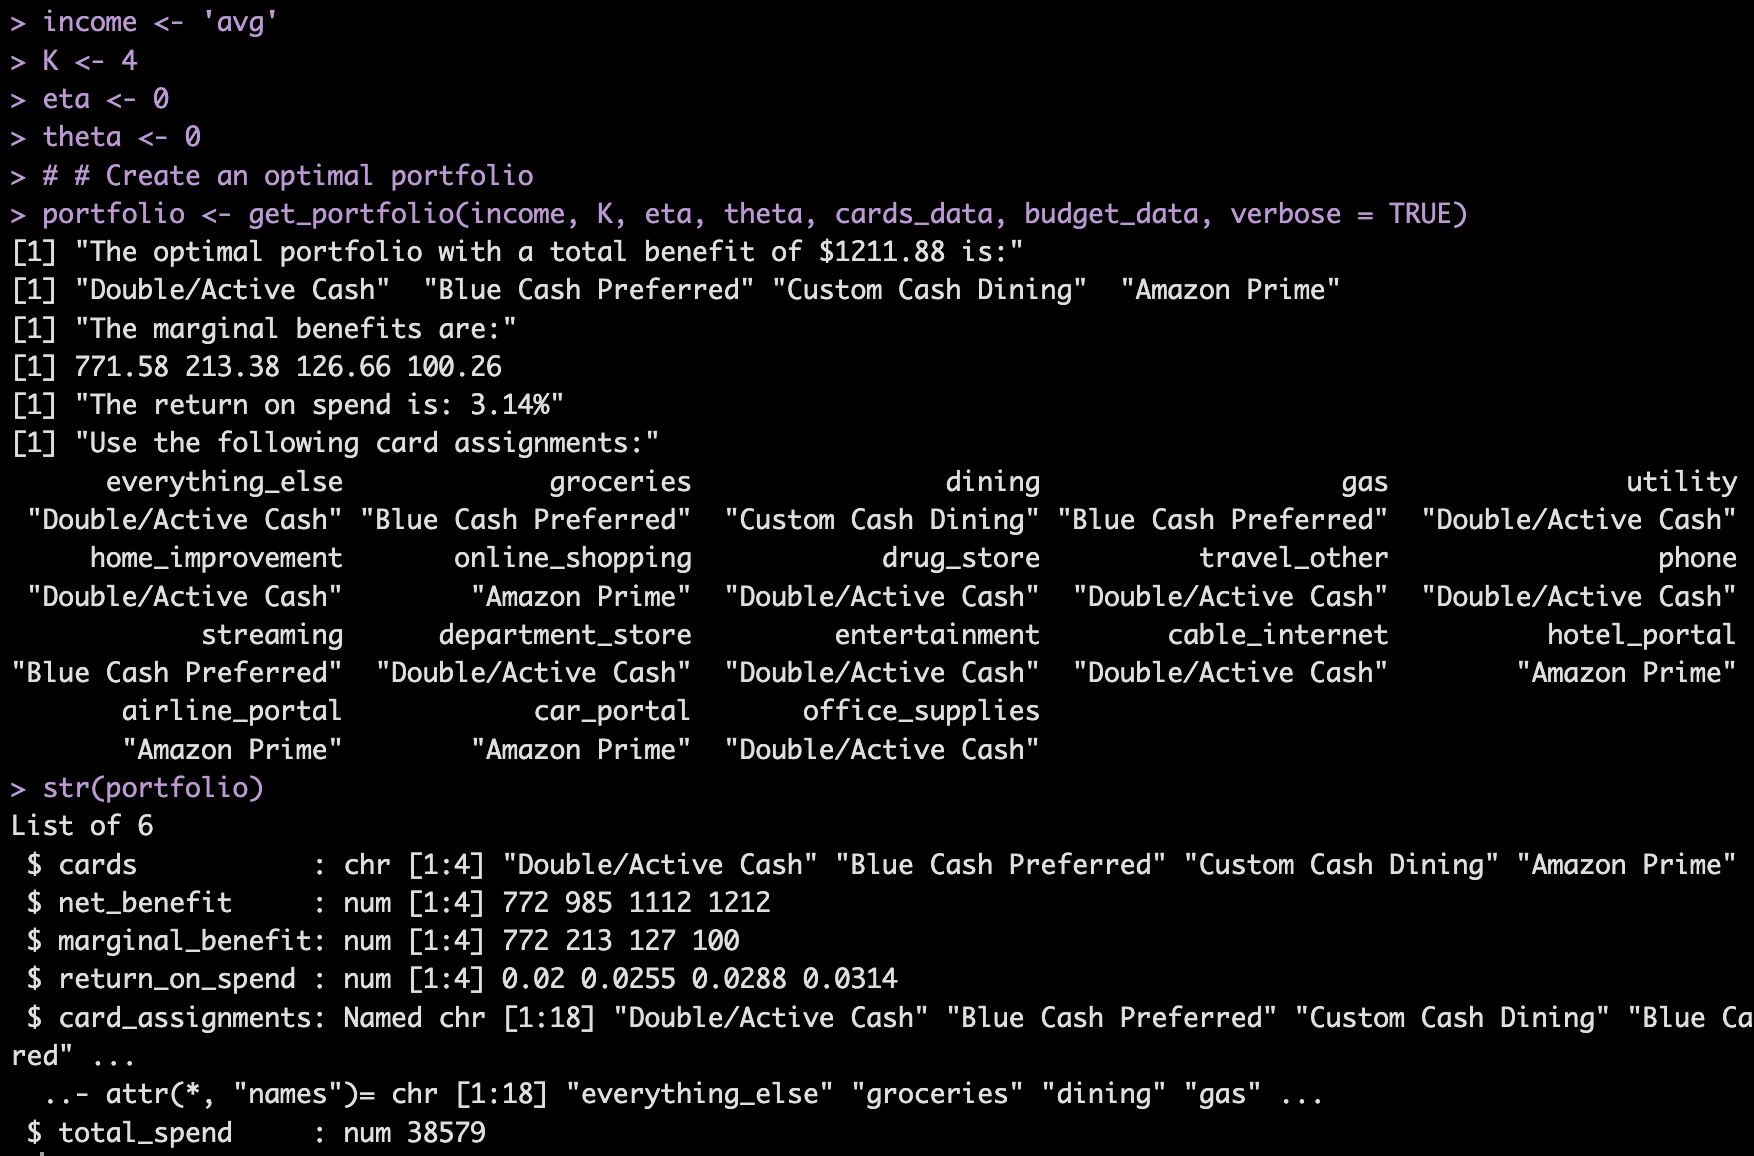
\includegraphics[width=1\textwidth]{../Misc/RCode_portfolio_output1.png}
    \end{center}
\end{frame} 

\begin{frame}{\sR\ Code output for \texttt{get\_portfolio}}
    \begin{itemize}
        \item Different user input, different output
    \end{itemize}
    \begin{center}
        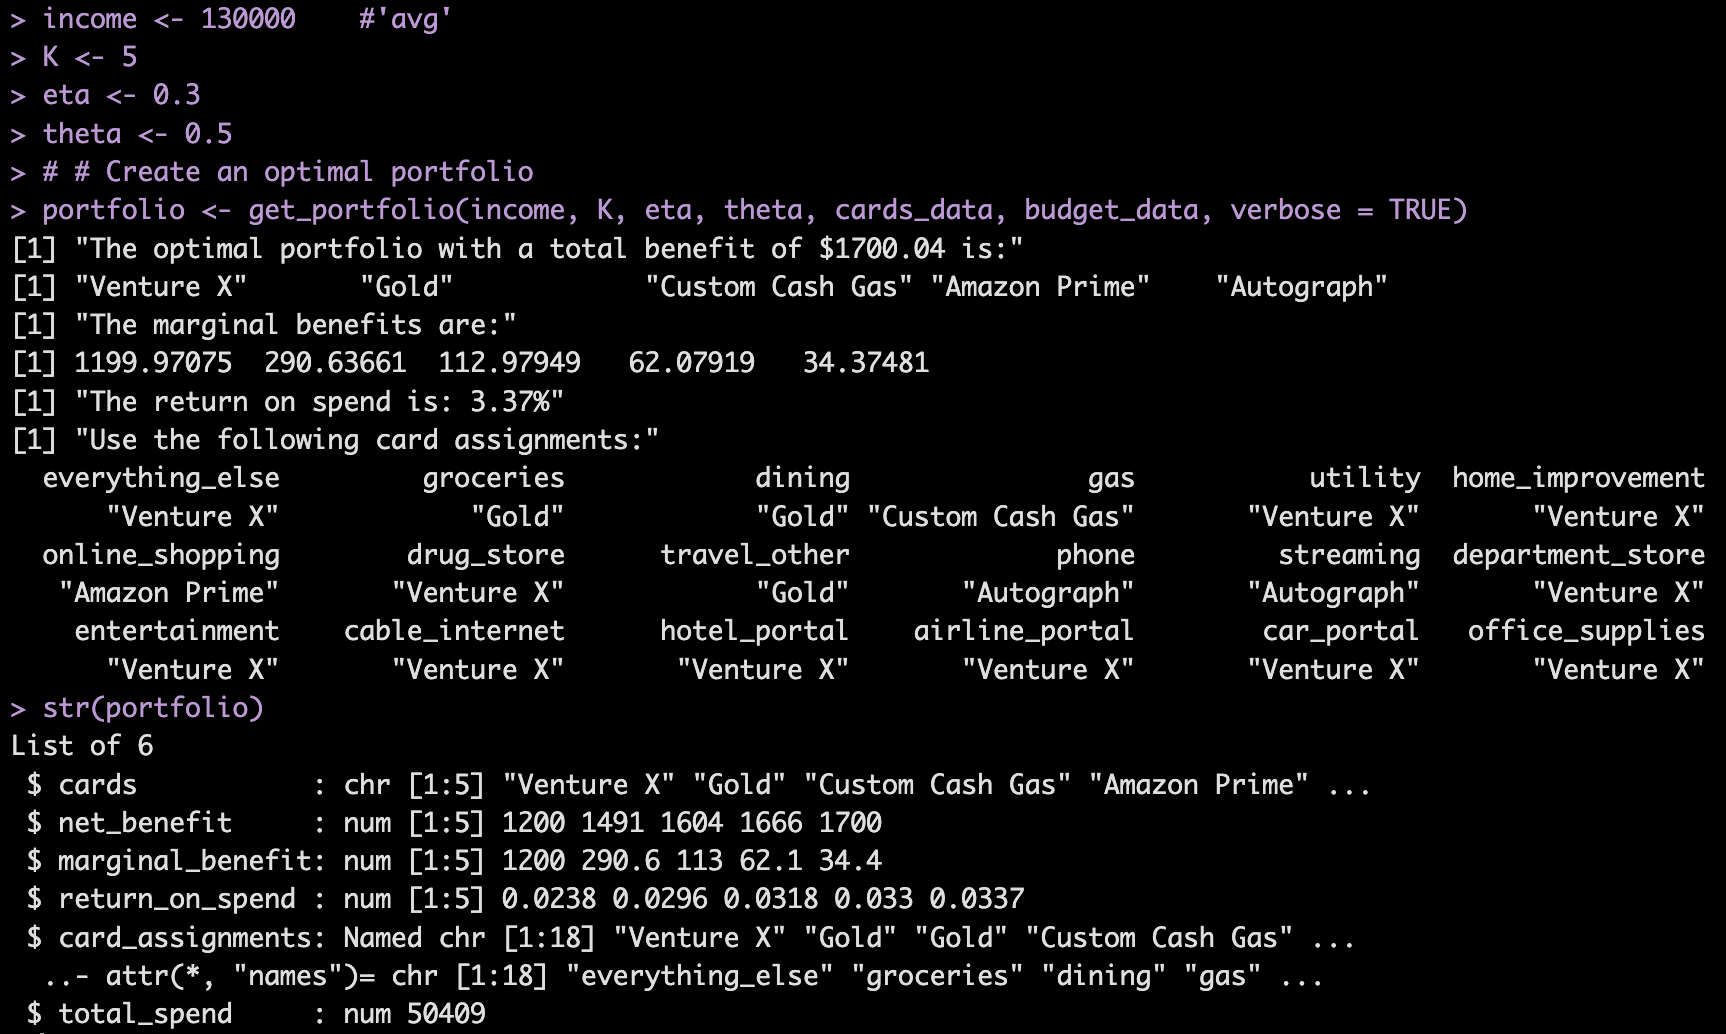
\includegraphics[width=1\textwidth]{../Misc/RCode_portfolio_output2.png}
    \end{center}
\end{frame} 

\begin{frame}{Portfolios Visualized 1}
    \begin{center}
        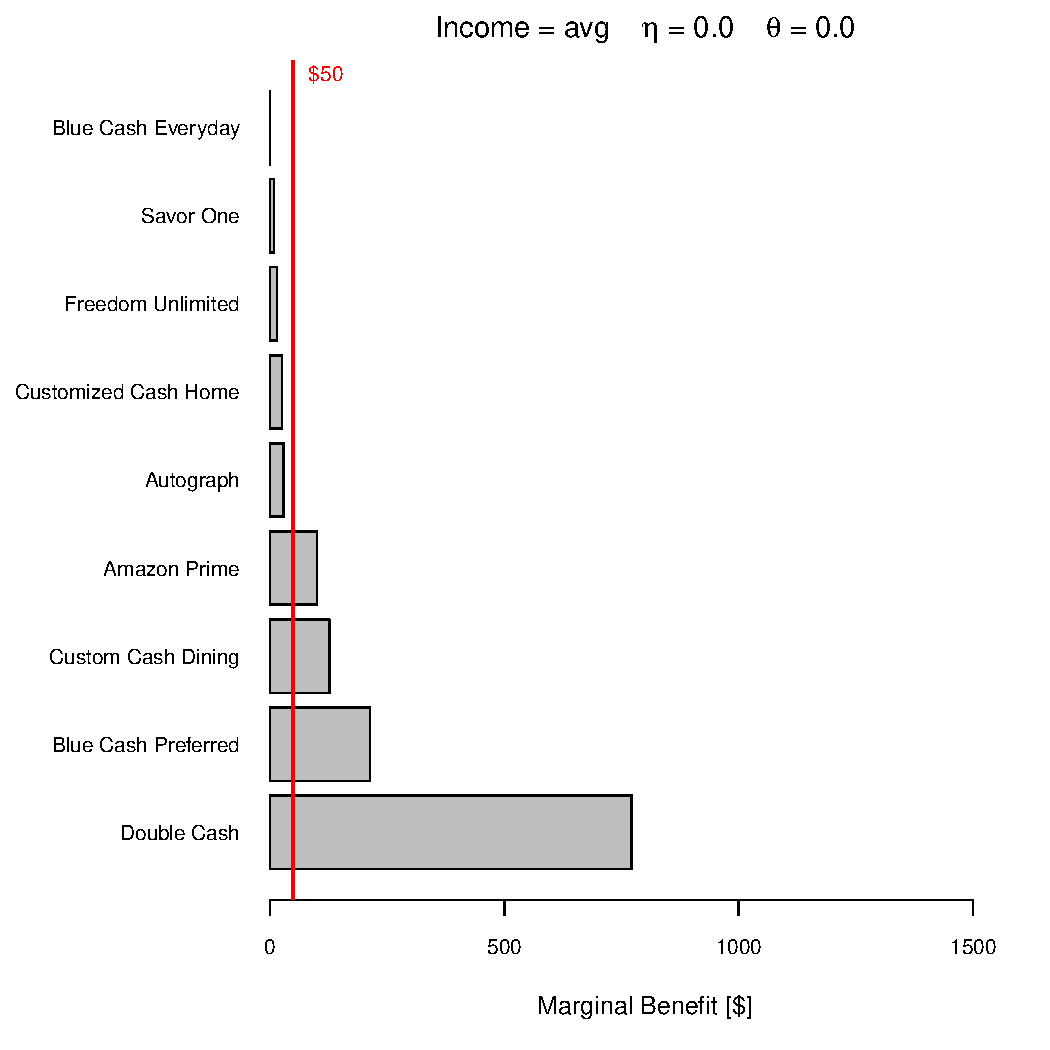
\includegraphics[width=0.9\textheight]{../Figures/Portfolio_avg_9_0_0.pdf}
    \end{center}
\end{frame} 

\begin{frame}{Portfolios Visualized 2}
    \begin{center}
        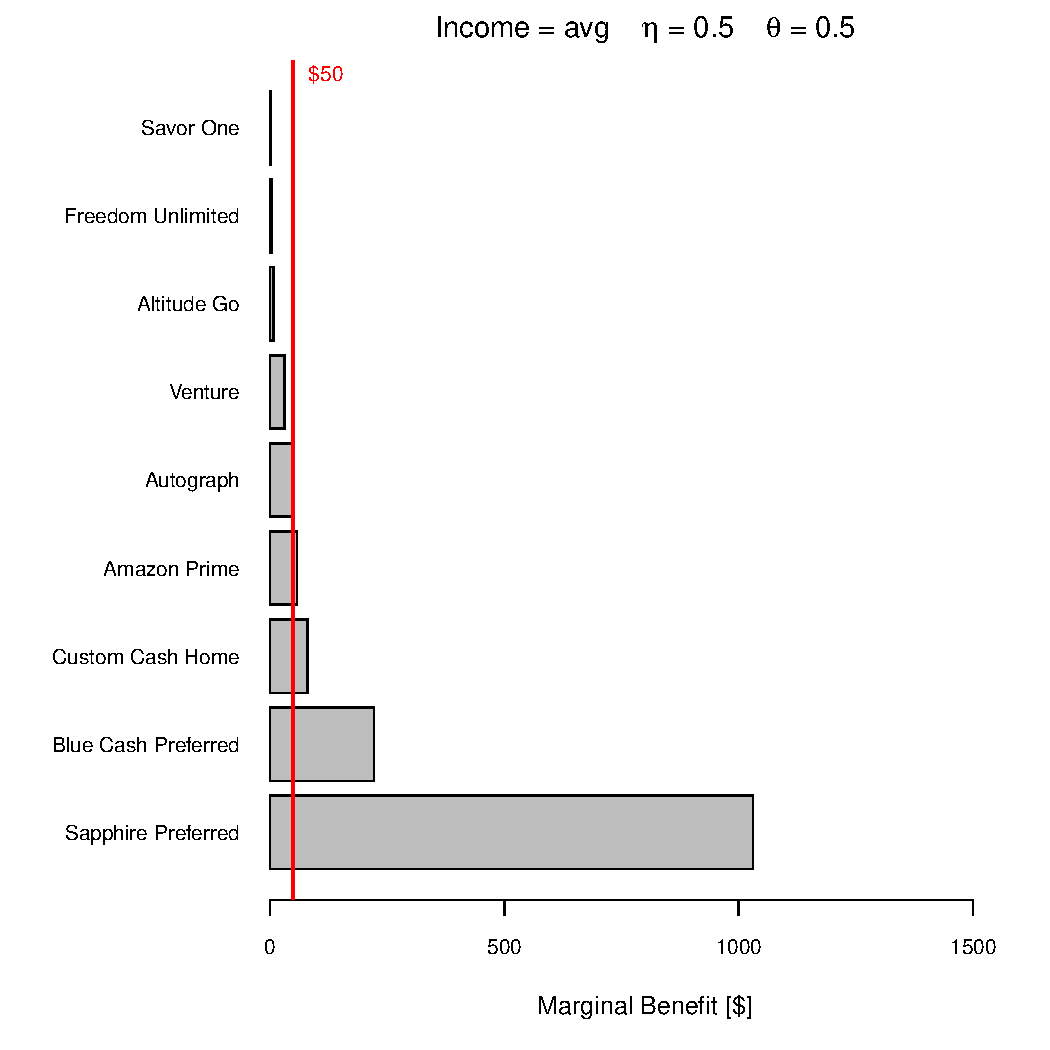
\includegraphics[width=0.9\textheight]{../Figures/Portfolio_avg_9_05_05.pdf}
    \end{center}
\end{frame} 

\begin{frame}{Portfolios Visualized 3}
    \begin{center}
        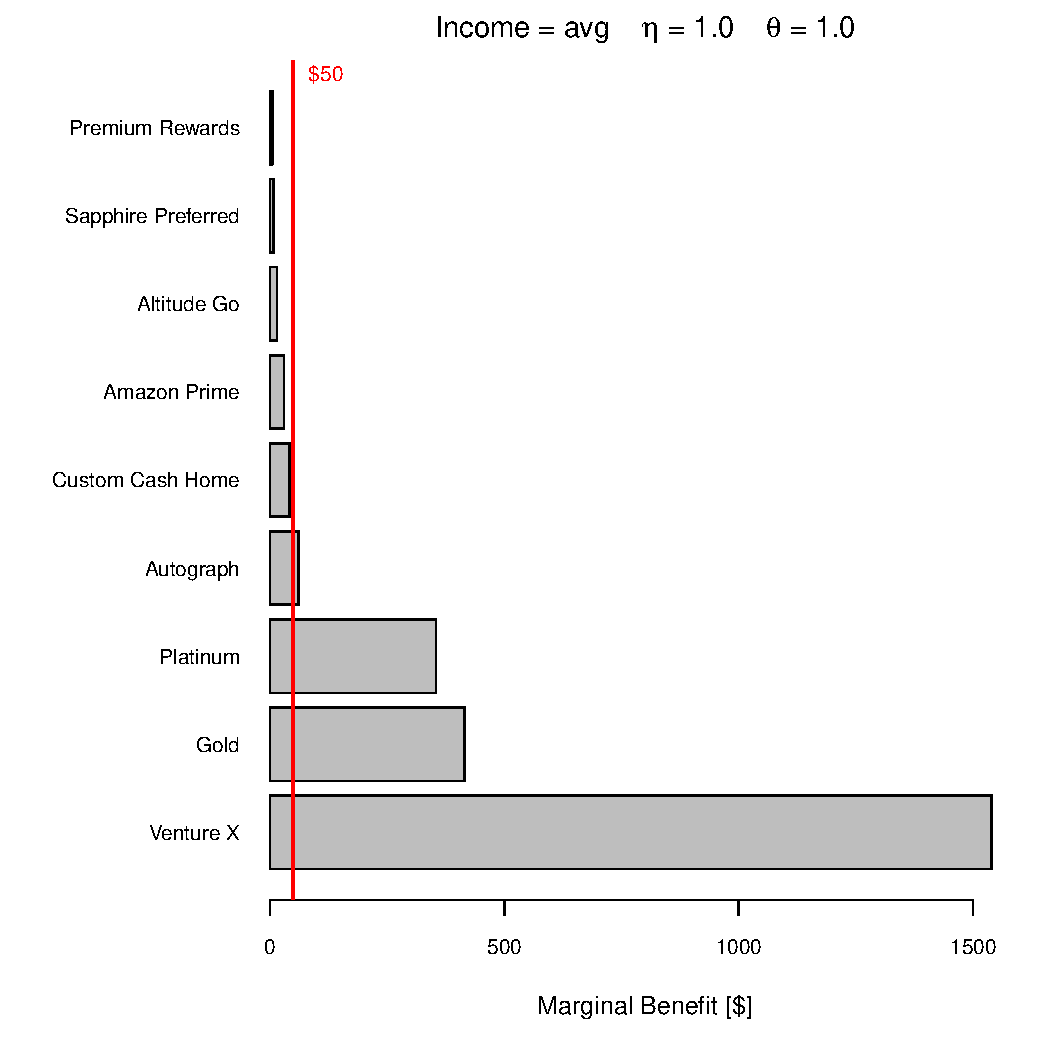
\includegraphics[width=0.9\textheight]{../Figures/Portfolio_avg_9_1_1.pdf}
    \end{center}
\end{frame} 


\section{Sensitivity Analysis}

\subsection{Number of Cards}

\begin{frame}{Number of Cards}
    \begin{columns}[c]
        \begin{column}{0.7\textwidth}
            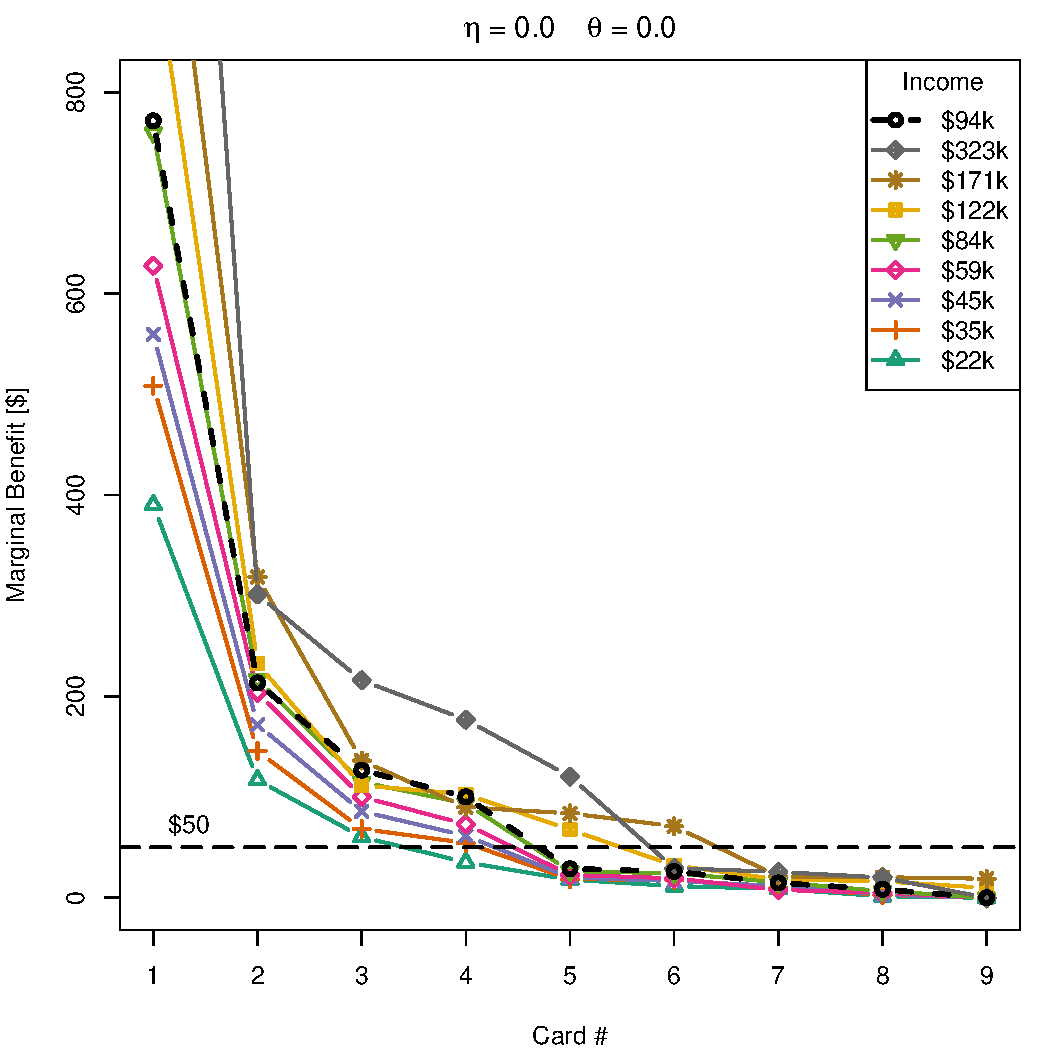
\includegraphics[width=0.9\textheight]{../Figures/MBvsKvsIncome_0_0.pdf}
        \end{column}
        \begin{column}{0.3\textwidth}
            \centering
            Four or five cards seems a reasonable choice for most people.
        \end{column}
    \end{columns}
\end{frame} 

\begin{frame}{Number of Cards}
    \begin{columns}[c]
        \begin{column}{0.7\textwidth}
            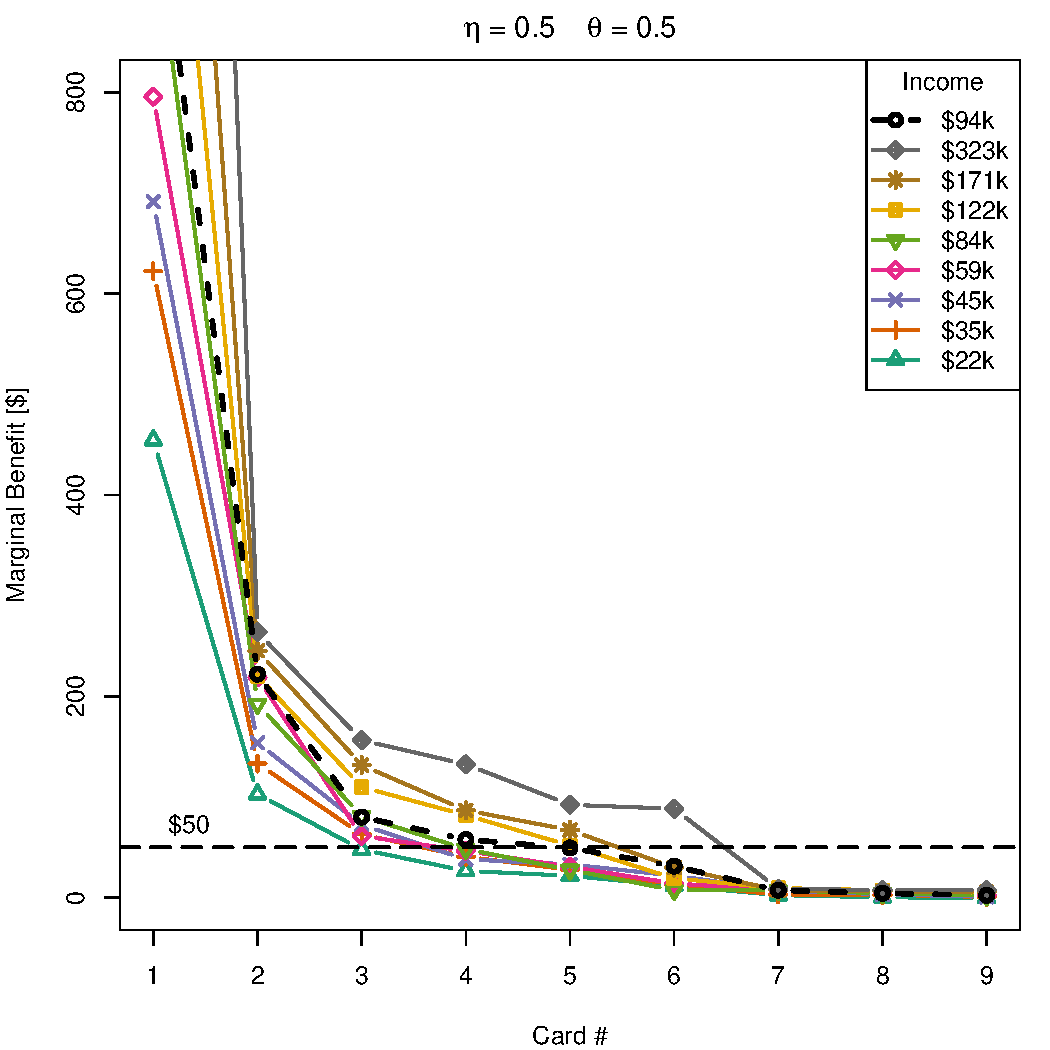
\includegraphics[width=0.9\textheight]{../Figures/MBvsKvsIncome_05_05.pdf}
        \end{column}
        \begin{column}{0.3\textwidth}
            \centering
            Four or five cards seems a reasonable choice for most people.
        \end{column}
    \end{columns}
\end{frame} 

\begin{frame}{Number of Cards}
    \begin{columns}[c]
        \begin{column}{0.7\textwidth}
            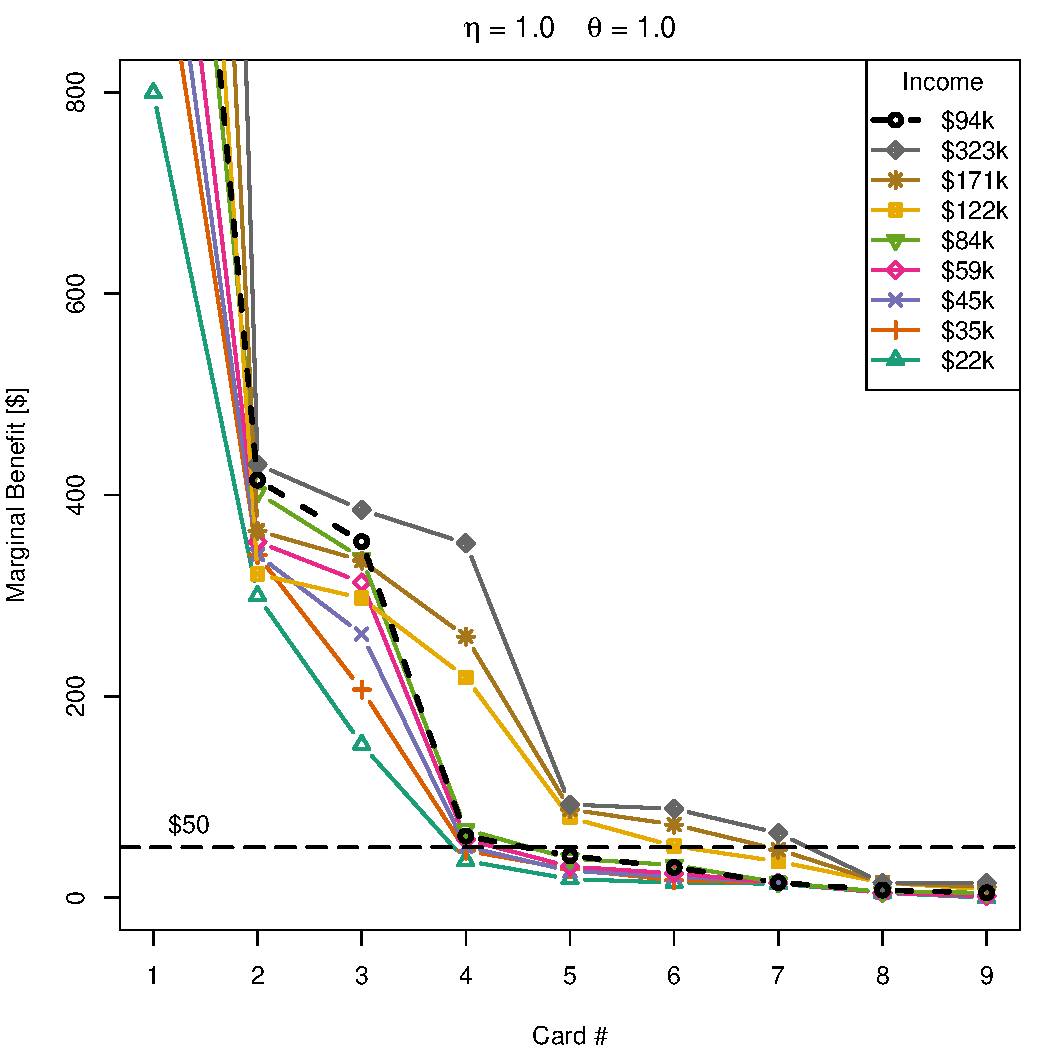
\includegraphics[width=0.9\textheight]{../Figures/MBvsKvsIncome_1_1.pdf}
        \end{column}
        \begin{column}{0.3\textwidth}
            \centering
            Wealthier people can justify annual fees more easily, unlocking better multipliers or benefits.\\
            \bigskip
            There is a potential issue with overlapping benefits.
            % Premium cards add lounge access AND global entry AND Clear credits
            % multiple times!
            % Might need to split out benefits over separate columns?
        \end{column}
    \end{columns}
\end{frame} 


\subsection{Net Benefit}

% Net Benefit vs Income
\begin{frame}{Net Benefit}
    \begin{columns}[c]
        \begin{column}{0.7\textwidth}
            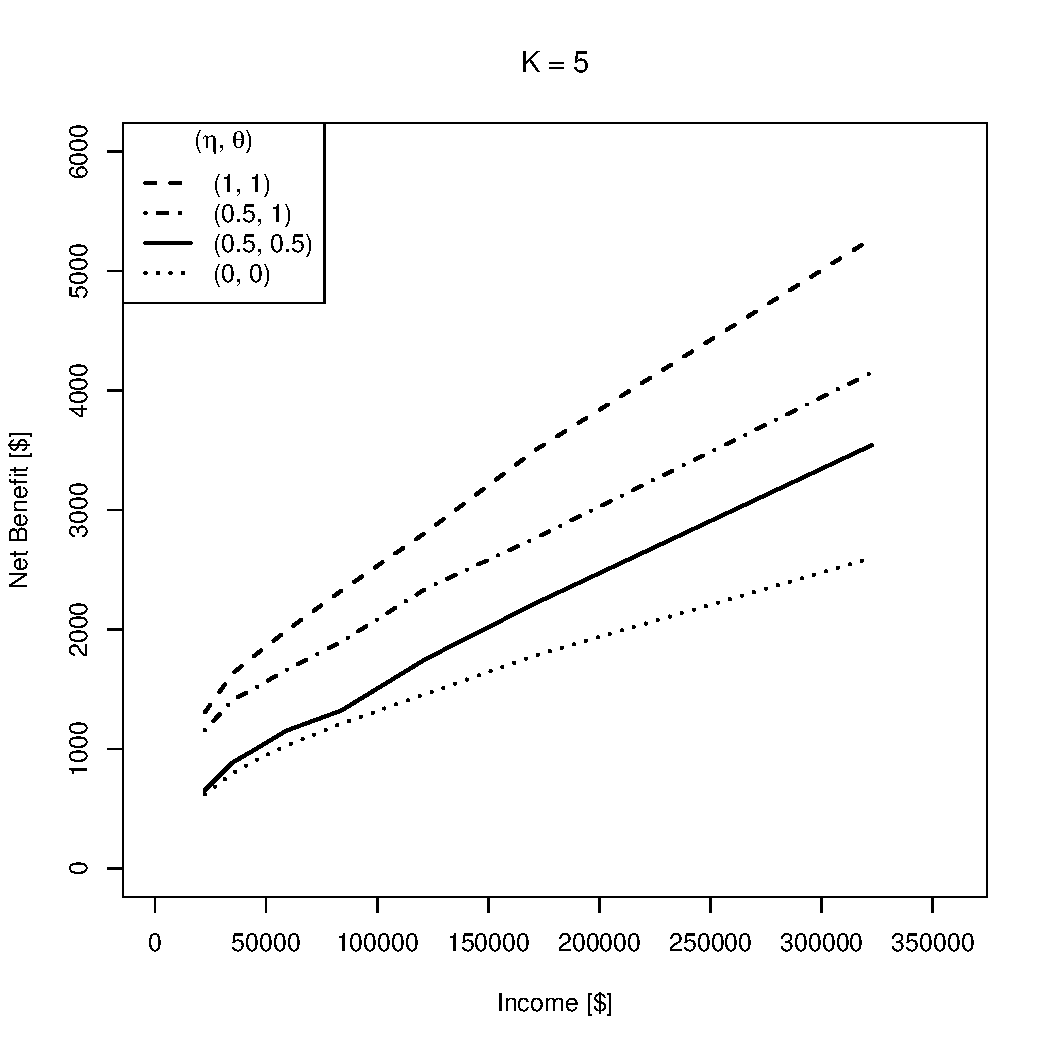
\includegraphics[width=0.9\textheight]{../Figures/NBvsIncome_K5.pdf}
        \end{column}
        \begin{column}{0.3\textwidth}
            \centering
            Shows the range of potential total benefit when using 5 cards.
        \end{column}
    \end{columns}
\end{frame} 

\subsection{Return on Spend}

% Show Return on Spend % vs number of cards and income
% Benefits become more lucrative for lower incomes
\begin{frame}{Return on Spend}
    \begin{columns}[c]
        \begin{column}{0.7\textwidth}
            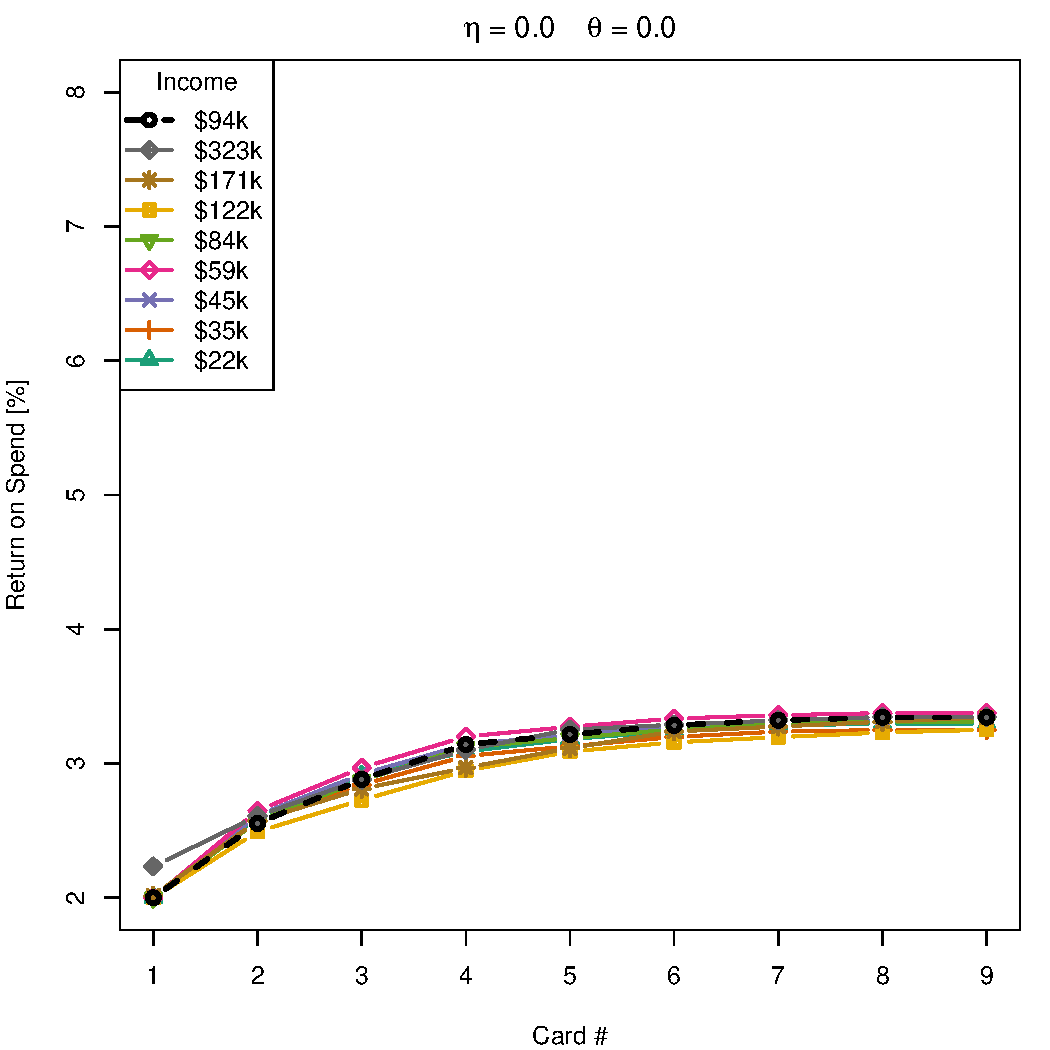
\includegraphics[width=0.9\textheight]{../Figures/ROSvsKvsIncome_0_0.pdf}
        \end{column}
        \begin{column}{0.3\textwidth}
            \centering
            Everyone could increase their Return on Spend from 2\% to 3.2--3.3\% by using 5--6 cards.
        \end{column}
    \end{columns}
\end{frame} 

\begin{frame}{Return on Spend}
    \begin{columns}[c]
        \begin{column}{0.7\textwidth}
            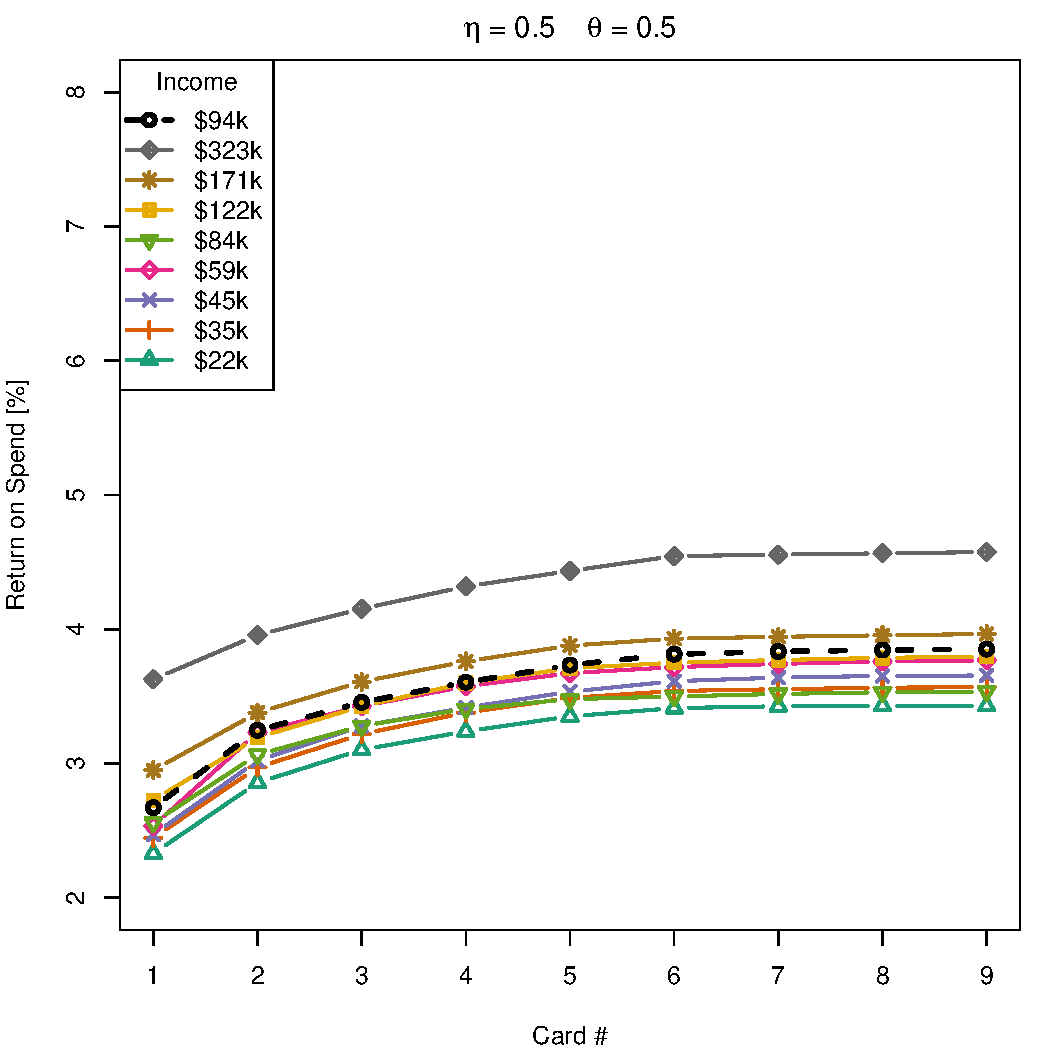
\includegraphics[width=0.9\textheight]{../Figures/ROSvsKvsIncome_05_05.pdf}
        \end{column}
        \begin{column}{0.3\textwidth}
            \centering
            Travel cards most benefit the wealthy.
            % Sapphire Reserve 1 card wealthy solution 3.6%
        \end{column}
    \end{columns}
\end{frame} 

\begin{frame}{Return on Spend}
    \begin{columns}[c]
        \begin{column}{0.7\textwidth}
            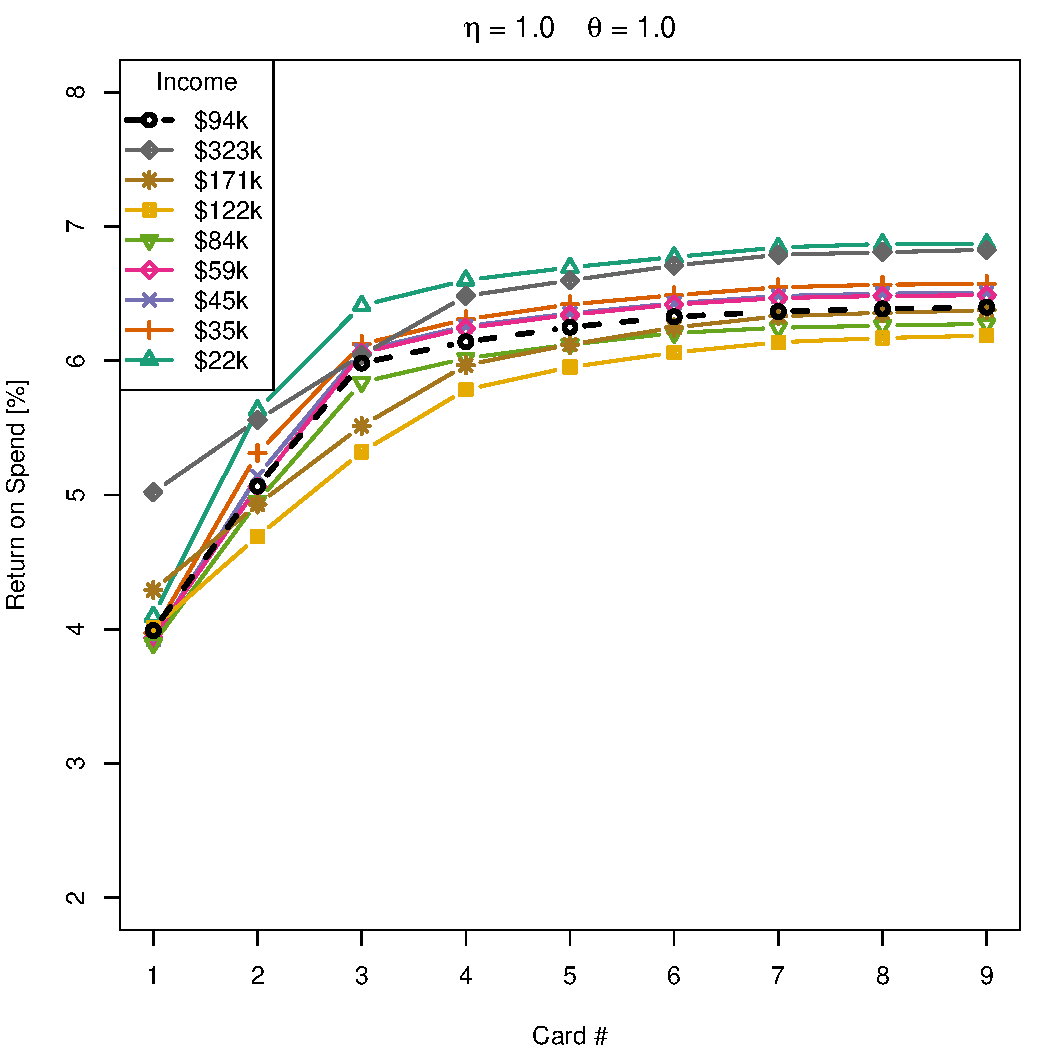
\includegraphics[width=0.9\textheight]{../Figures/ROSvsKvsIncome_1_1.pdf}
        \end{column}
        \begin{column}{0.3\textwidth}
            \centering
            Here we expose the limits of the model\ldots
            % Premium cards add lounge access AND global entry AND Clear credits
            % multiple times!
            % Need to split out benefits over separate columns and not allow
            % overlap!
        \end{column}
    \end{columns}
\end{frame} 

\begin{frame}{We broke our model}
    \begin{itemize}
        % Low incomes probably also don't qualify for premium cards...
        \item<+-> ``Low incomes should just stack all the premium, high-fee travel cards and travel, using all the benefits multiple times!''
        \item<+-> I will need to categorize the benefits and make them single-use\ldots 
    \end{itemize}
    \begin{center}
        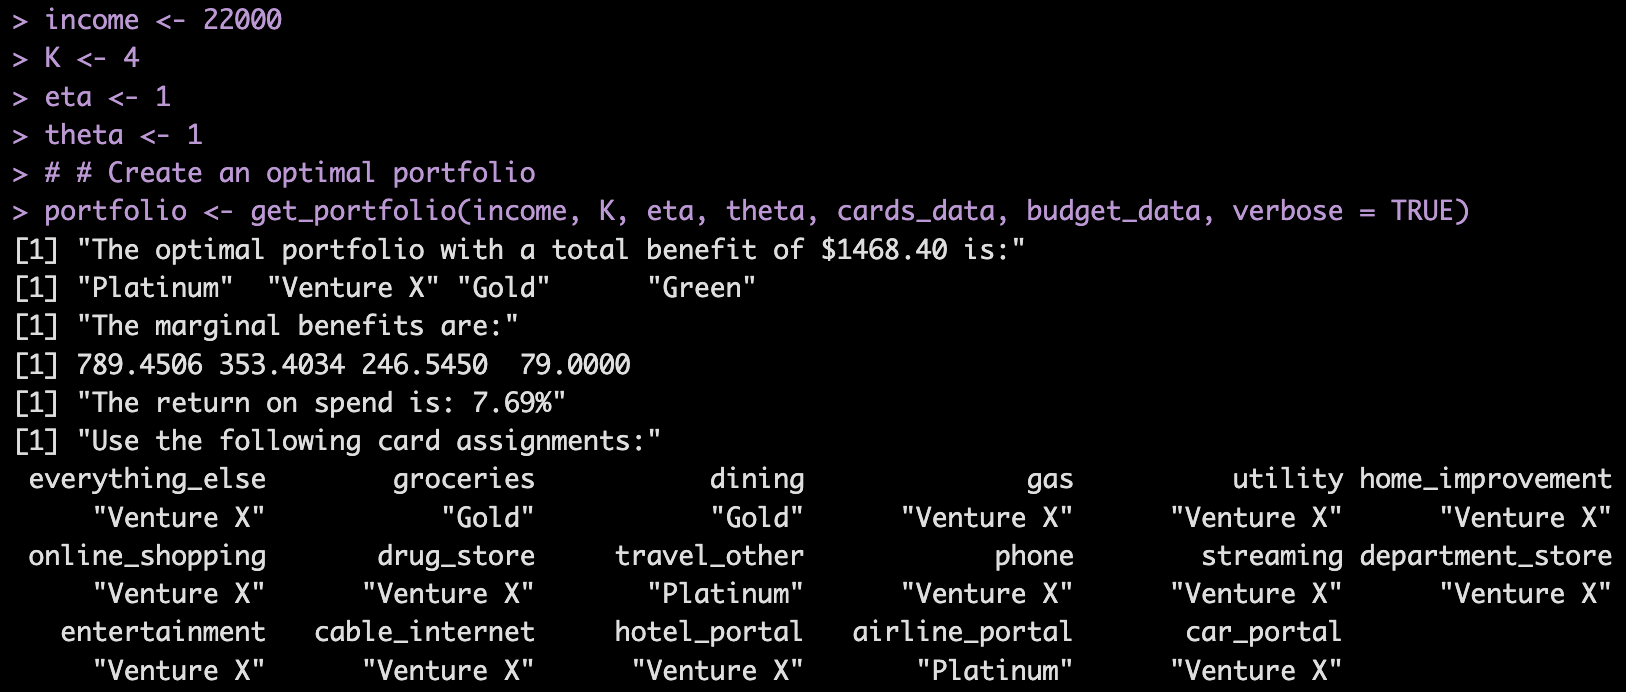
\includegraphics[width=1\textwidth]{../Misc/ModelLimit.png}
    \end{center}
\end{frame} 

\begin{frame}{Return on Spend}
    \begin{itemize}
        \item A different way of comparing two incomes
        \item All these figures need updating after fixing the benefits (easy using shell scripts!)
    \end{itemize}
    \begin{columns}[c]
        \begin{column}{0.5\textwidth}
            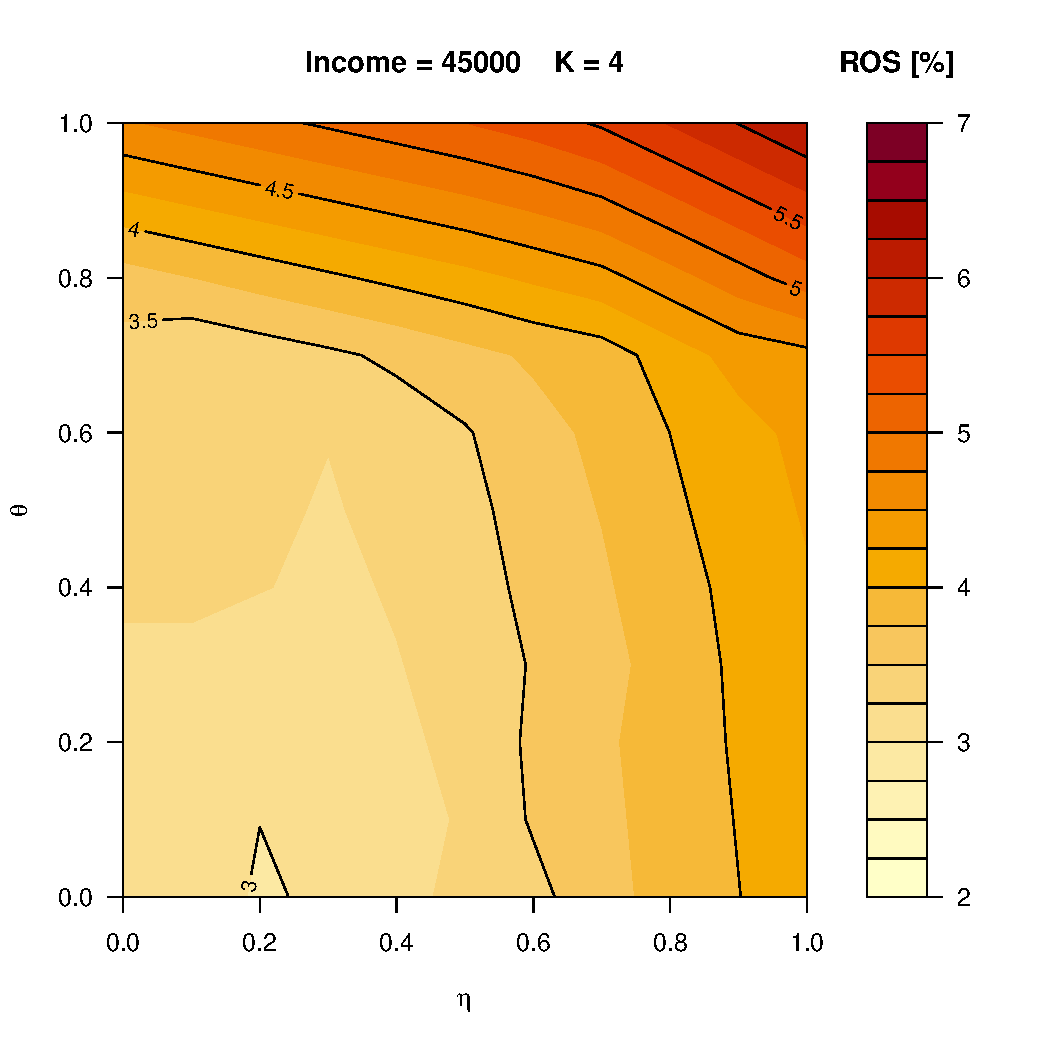
\includegraphics[width=1.1\textwidth]{../Figures/ROSvsEtaTheta_K5_Inc45k.pdf}
        \end{column}
        \begin{column}{0.5\textwidth}
            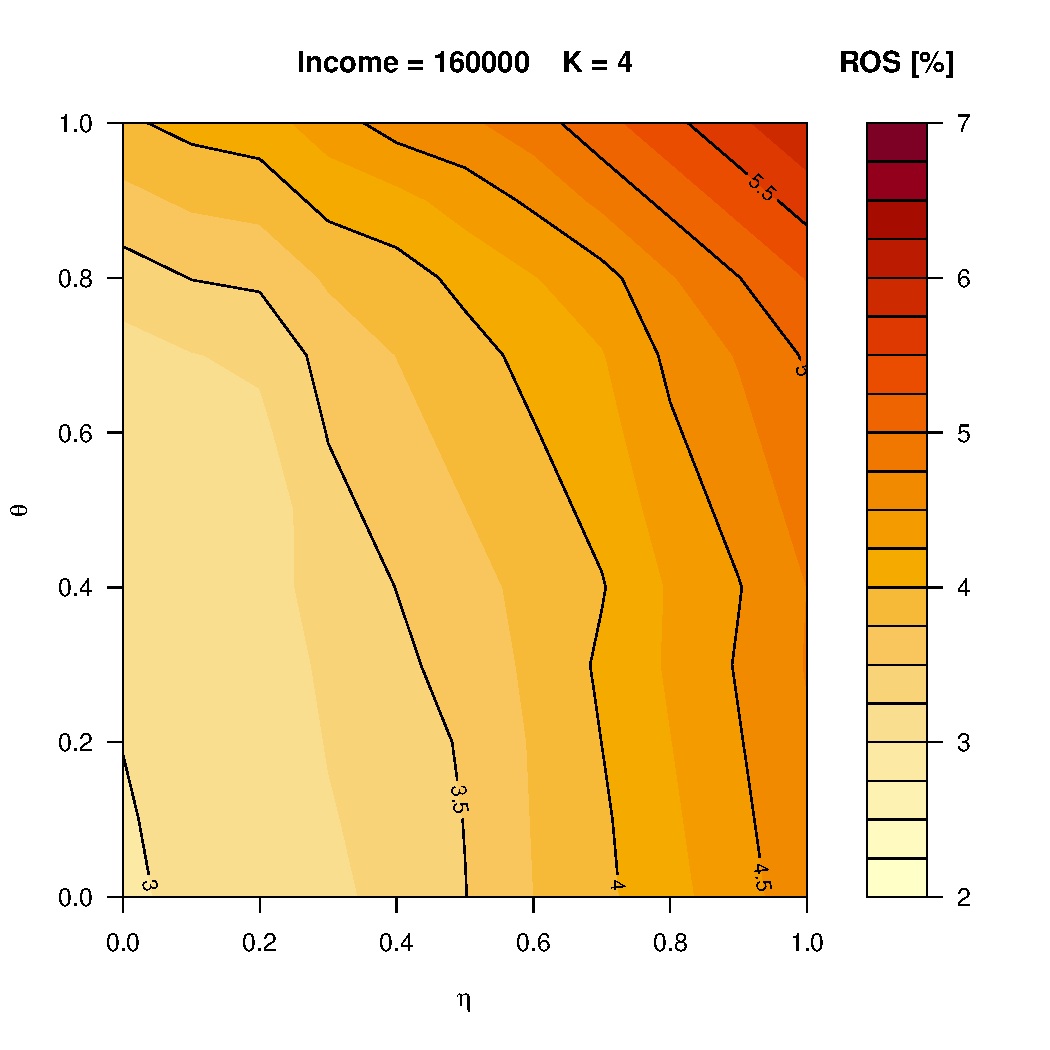
\includegraphics[width=1.1\textwidth]{../Figures/ROSvsEtaTheta_K5_Inc160k.pdf}
        \end{column}
    \end{columns}
\end{frame} 

\section{Summary \& Conclusions}

% Potential problem: overlapping benefits for wealthy people and high annual fee cards.

\begin{frame}
    \frametitle{Summary \& Conclusions}
    \begin{itemize}
        \item Algorithm works, and produces realistic portfolios for a variety of inputs (when benefits are turned off)
        \bigskip
        \item Spending on $\sim$5 cards seems to be the sweet spot for most people (ROS of $\sim$3.2\%, assuming base valuations and no benefits)
        \bigskip
        \item The Sensitivity Analysis exposed a flaw in the treatment of benefits, which can be fixed in the same way we deal with spend categories
        \bigskip
        \item Next Steps: fix overlapping benefits, sample realistic incomes (Monte Carlo), build Shiny App
    \end{itemize}
\end{frame}

\begin{frame}
    \vfill
    \centering
    \begin{beamercolorbox}[sep=8pt,center,shadow=true,rounded=true]{title}
      \usebeamerfont{title}Thank You!
    \end{beamercolorbox}
    \vfill
\end{frame}

\section*{Appendix}

\begin{frame}
    \vfill
    \centering
    \begin{beamercolorbox}[sep=8pt,center,shadow=true,rounded=true]{title}
      \usebeamerfont{title}Extra Slides
    \end{beamercolorbox}
    \vfill
\end{frame}


\begin{frame}{\texttt{get\_portfolio} 1/3}
    \begin{center}
        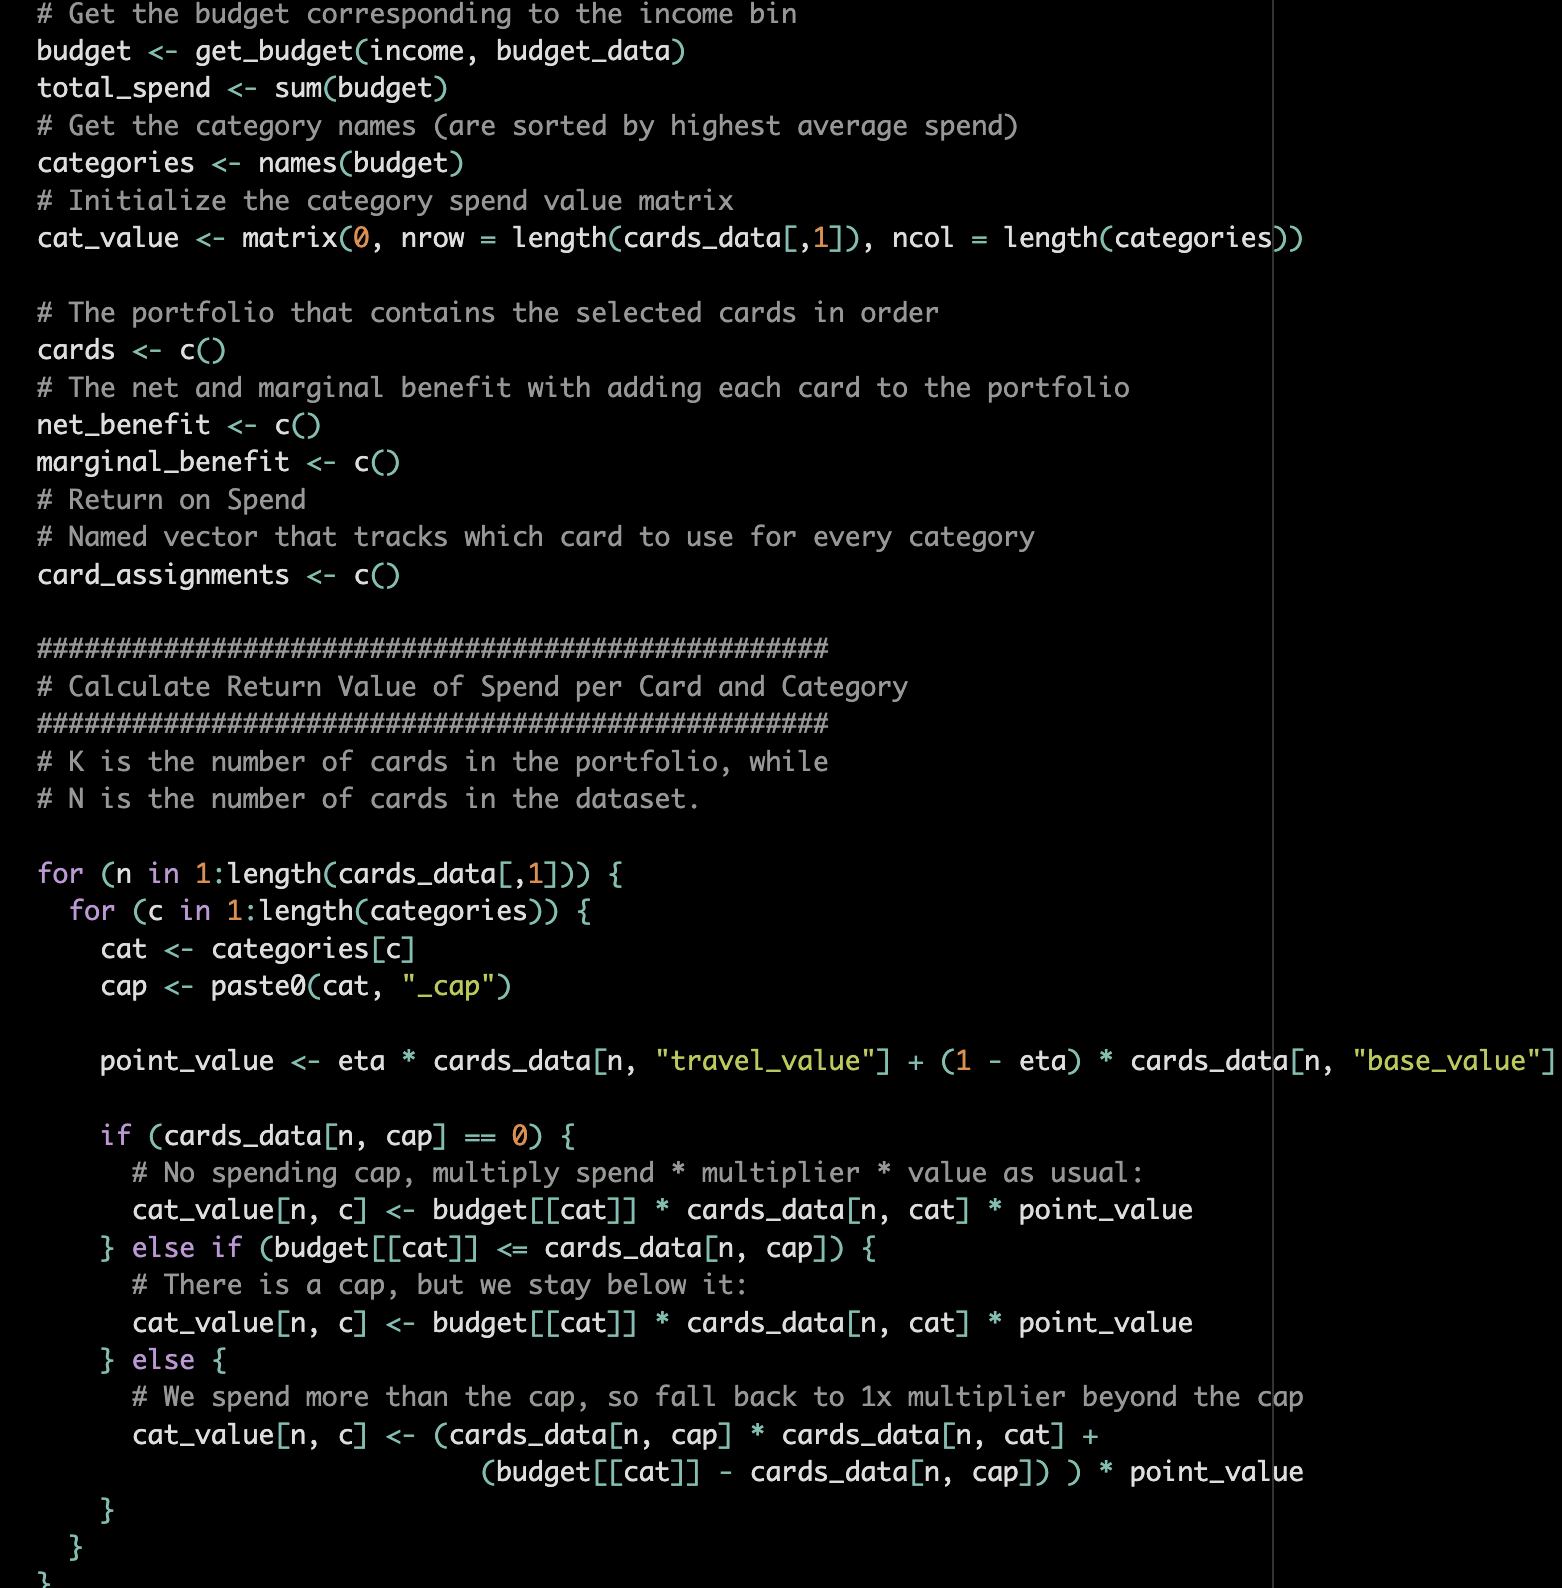
\includegraphics[width=0.9\textheight]{../Misc/RCode_portfolio1.png}
    \end{center}
\end{frame} 
\begin{frame}{\texttt{get\_portfolio} 2/3}
    \begin{center}
        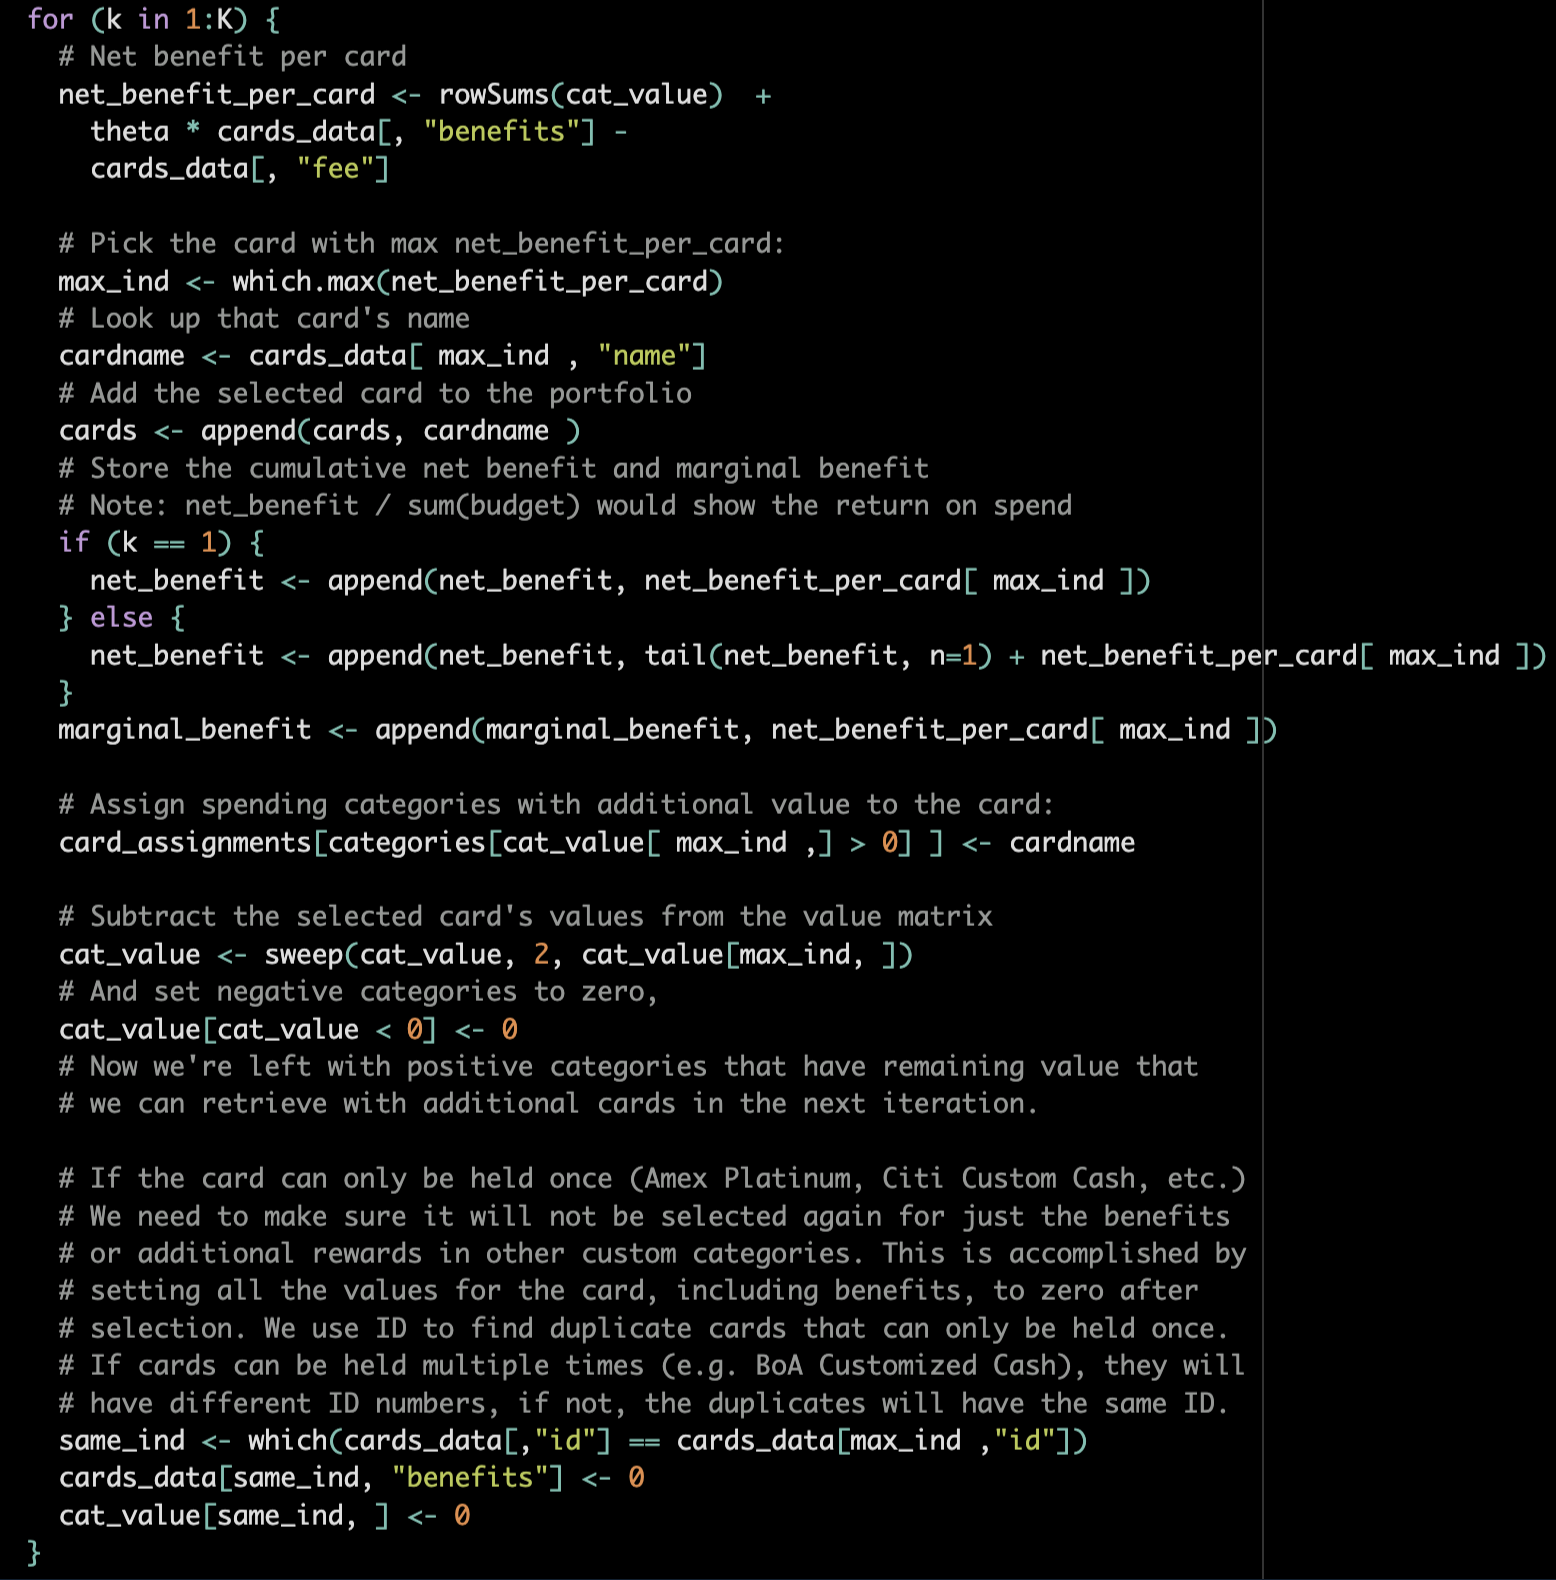
\includegraphics[width=0.9\textheight]{../Misc/RCode_portfolio2.png}
    \end{center}
\end{frame} 
\begin{frame}{\texttt{get\_portfolio} 3/3}
    \begin{center}
        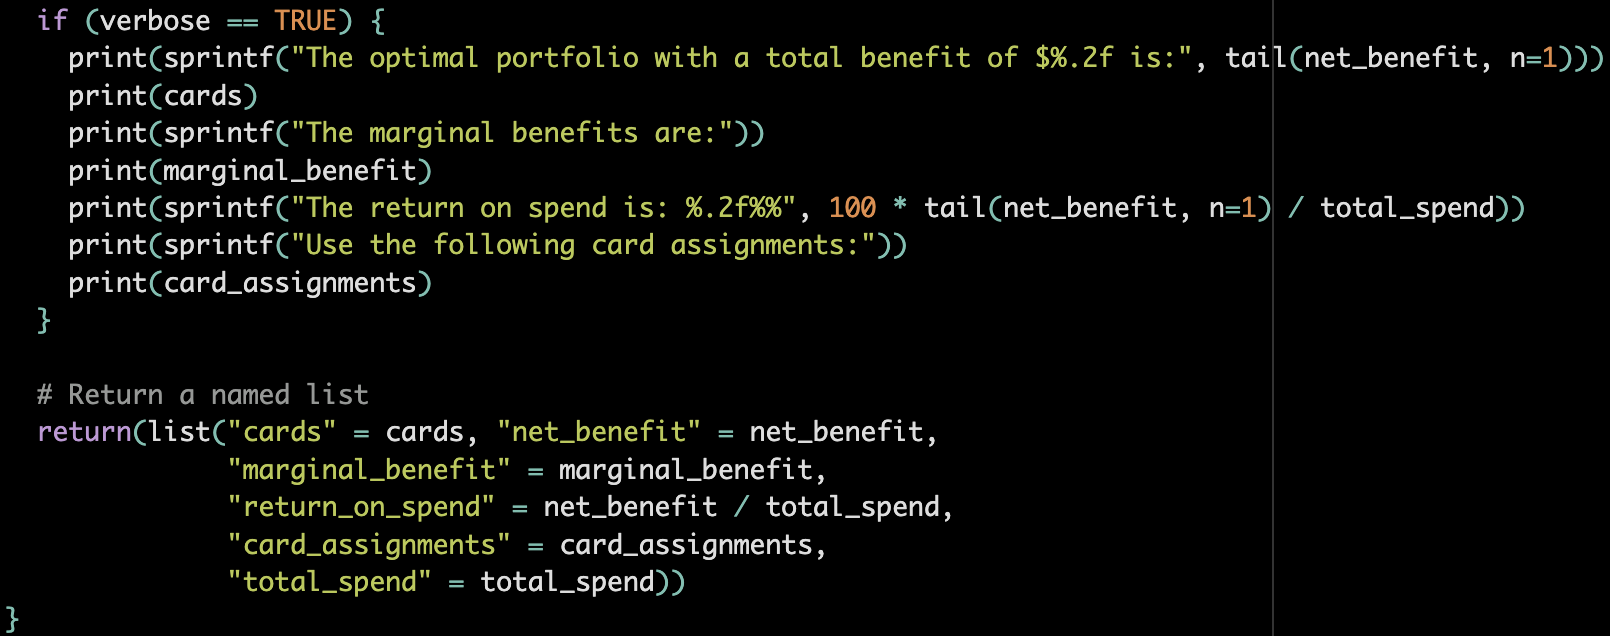
\includegraphics[width=0.9\textheight]{../Misc/RCode_portfolio3.png}
    \end{center}
\end{frame} 

% \begin{frame}{References}
%     \bibliographystyle{../chicago}
%     \bibliography{../References}
% \end{frame}    
